\usetikzlibrary{circuits.ee.IEC}
 
%%%%%%% Im Dokumentkopf %%%%%%%
% arrow source
\newcommand{\Bigrightarrow}{\mathord{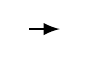
\begin{tikzpicture}[baseline=0ex, line width=1, scale=0.13, ->, >=latex]
%\draw (1,0) -- (1,2);
\draw[] (0,0) -- (3,0);
\end{tikzpicture}~}}
%
\tikzset{circuit declare symbol = arrow source}
\tikzset{set arrow source graphic ={draw,generic circle IEC, minimum size=5mm,info sloped=center:$\,\:\Bigrightarrow$}}
%%%%%%%%%%%%%%%%%%%%%%%%%%%%%%%%
 
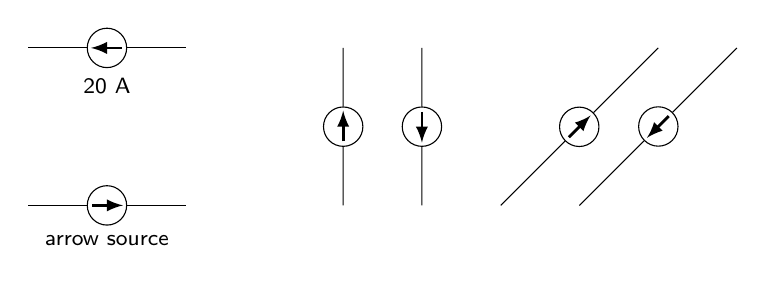
\begin{tikzpicture}[circuit ee IEC, font=\sffamily\footnotesize]
% arrow source
\draw (0,0) to [arrow source={info'={arrow source}}](2,0);
%Zeichenrichtung ändern
\draw (2,2) to [arrow source={info'={20 A}}](0,2);
%hochkant
\draw (4,0) to [arrow source](4,2);
\draw (5,2) to [arrow source](5,0);
%schräg
\draw (6,0) to [arrow source](8,2);
\draw (9,2) to [arrow source](7,0);
\end{tikzpicture}